\documentclass[10pt,letterpaper]{article}
\usepackage{spconf}
\usepackage[T1]{fontenc}
\usepackage{amsmath,amssymb,graphicx,booktabs,url}
\urlstyle{same}
\usepackage[hidelinks]{hyperref}
\hypersetup{pdftitle={ReCheck: Auditing Full-Progress Scores Against Executed Effects in LLM Agents},pdfauthor={Author details pending},pdfsubject={AI-assisted research working draft; not a submission-ready document}}
\title{ReCheck: Auditing Full-Progress Scores Against Executed Effects in LLM Agents}
% This file must be filled by the real author; the research is not anonymous.
\name{Author names pending}
\address{Department, institution, city, country pending \\
Contact email pending \\
{\fontsize{9}{10.8}\selectfont AI-generated research working draft; not for direct submission}}

\begin{document}
\maketitle
\begin{abstract}
Completion scores for tool-using agents need not certify the effects requested by users. We present ReCheck, a retrospective audit that links active requests to executed tool receipts and recorded state. In 576 public records from six task templates, we retain 64 full-progress/effect conflicts after contextual review: 62 reminders have incorrect calendar dates, and two were never created. These constitute 30.2\% of 212 full-progress reminder records, not a benchmark-wide error rate. A separate 960-record coverage finds no conflicting checked effect among 802 full-progress records with sufficient state evidence. Native scripted controls additionally show that historical achievement can survive later reversal in milestone scoring, while indiscriminate terminal checks reject authorized revisions. ReCheck preserves original scores, separates observed conflicts from unresolved semantics, and makes no model-ranking or treatment-effect claim. The findings motivate completion audits grounded in executed values and the temporal scope of user requests.

\end{abstract}
\begin{keywords}
Agent evaluation, tool use, benchmark auditing, temporal reasoning, outcome verification
\end{keywords}

\section{Introduction}
\label{sec:intro}
Stateful language-model agents must do more than describe a correct action: they must execute it on the intended object and produce the requested effect. ToolSandbox evaluates stateful interactions using intermediate and final milestones~\cite{toolsandbox}. Talk, Evaluate, Diagnose (TED) converts benchmark milestones into natural-language grading notes and evaluates progress with a model judge~\cite{ted}. These designs measure useful aspects of behavior, but their scores should not automatically be interpreted as certificates of task completion.

Consider a saved interaction in which the user requests a reminder for next Friday. The time-conversion receipt says that the current day is Tuesday, September 16, 2025. The agent creates a reminder for Saturday, September 20, yet the source reports full progress. In another interaction, a request for tomorrow produces a reminder timestamp from 2023 despite a recorded current clock in 2025. Both have concrete execution evidence, rather than merely incorrect explanatory text.

We study a narrow question: \emph{when a recorded evaluation reports full progress, does the observable effect satisfy a necessary condition of the still-active user request?} ReCheck is an execution-grounded audit protocol, not a new planning algorithm or a replacement leaderboard. Its contribution is a trace-indexed empirical analysis of value and execution mismatches in a specific public corpus, complemented by native controls that expose the limits of purely historical or terminal checks. We retain negative findings, legitimate revisions, and unknown cases instead of treating every discrepancy as an agent failure.

Our primary audit covers 576 saved records across six templates and identifies 64 conservatively retained full-progress/effect conflicts. Separately, 960 setting/contact records provide a negative coverage check. Fifty scripted trajectories over nine public ToolSandbox tasks examine temporal scope; these are not additional model samples. Original source scores remain unchanged throughout.

\section{Related Work and Study Position}
\label{sec:related}
LLM-as-a-judge research documents both useful human agreement and judge limitations~\cite{judge}. TED develops user-aware, subgoal-based progress metrics and error analysis~\cite{ted}; its limitations explicitly acknowledge that effects absent from a trajectory cannot be verified. Our audit concerns saved records with inspectable receipts and state. It does not establish which state fields the original judge received, or whether a mismatch arose in rubric conversion, context construction, or judging.

Benchmark-validity auditing is not itself new. Vaghasiya et al.~\cite{validity} audit four tool-calling benchmark families and propose separating invocation, completion, and outcome verification. Wang et al.~\cite{aba} study automated auditing across heterogeneous benchmark artifacts. Our study adds reproducible evidence of calendar-value and non-execution conflicts in the public SAP/TED ToolSandbox adaptation, while accounting for user revisions and ambiguous batch boundaries.

TimeBench documents difficulties with temporal reasoning~\cite{timebench}. We instead ask whether a completion score remains high \emph{despite} an observable temporal error. ToolSandbox's historical milestone matching is intentionally path-flexible~\cite{toolsandbox}; our temporal controls therefore test both missed final reversals and the opposite error of rejecting legitimate revisions. The two evaluation systems and their metrics are analyzed separately.

\section{Execution-Grounded Audit Protocol}
\label{sec:method}
\subsection{Evidence and the object being measured}
Let a saved interaction contain user messages $u$, structured action proposals $a$, tool receipts $r$, and available state snapshots $s$. For a task, we select a limited, necessary effect predicate $P$ from its documented request, and inspect later user messages for explicit revisions. We denote the resulting active requirement by $u^*$. Each auditable record links
\begin{equation}
 u^* \longleftrightarrow a_{\mathrm{id}}
 \longleftrightarrow r_{\mathrm{id}}
 \longleftrightarrow s_{\mathrm{object}} .
\label{eq:chain}
\end{equation}
Matching call identifiers and object identifiers establishes where the evidence came from; it does not itself establish correctness. Ordinary assistant text that resembles a tool call is not execution evidence. Successful creation is also distinct from creation with the requested value.

The local verdict is three-valued:
\begin{equation}
V_i=\begin{cases}
1,&\text{supported and consistent with }P(u_i^*,s_i),\\
0,&\text{supported contradiction of }P(u_i^*,s_i),\\
?,&\text{insufficient or unresolved evidence}.
\end{cases}
\label{eq:verdict}
\end{equation}
For source progress $q_i$, a reviewed conflict is
\begin{equation}
D_i=\mathbf{1}[q_i=1\ \land\ V_i=0].
\label{eq:conflict}
\end{equation}
A positive local verdict is \emph{not} full task success: unexamined side effects, other subgoals, and communication requirements may still fail. Conversely, $q_i<1$ with a correct local effect is not automatically a false negative. We use $D_i$ only to report conflicts with completion interpretations of a full source score.

\subsection{Reconstruction and contextual review}
We interpret each observed database namespace update as a complete table snapshot, not a row-level patch. Multiple tool receipts may contain the same batch-end state and may appear in a different order from proposals. We therefore check observed batch boundaries, not invented states between calls. Missing or contradictory evidence remains unknown. Repeated transcript appearances are not additional tool invocations.

Reminder predicates connect the requested content and date to the actual created object. Relative dates use the recorded current-time receipt, not a file-export date. Conversion receipts establish the observed clock mapping. For next Friday, initial screening accepts either of the next two future Fridays; a separate conservative check rejects only past dates or non-Fridays, without using the hour. Thus the retained calendar conflicts do not depend on choosing one narrow interpretation of next Friday. Explicit unresolved user time zones and clock ambiguities are excluded from the retained set.

The parser uses finite, documented content variants and abstains on unresolved expressions. Candidate review reads original user and assistant messages, calls, receipts, and stored values. Explicit user rescheduling changes the active requirement; a routine acknowledgement does not by itself do so. Candidate decisions received author review; no inter-rater agreement is claimed.

\subsection{Temporal scope as a separate control}
For a requirement active over an interval $I_j=[a_j,b_j]$, three different checks are possible:
\begin{align}
H_j &= \mathbf{1}[\exists t\in I_j:P_j(s_t)],\\
T_j &= \mathbf{1}[P_j(s_{b_j})],\\
G_j &= \mathbf{1}[\forall t\in I_j:P_j(s_t)].
\label{eq:scope}
\end{align}
Historical achievement $H_j$ does not imply terminal validity $T_j$, while an invariant $G_j$ is stronger still. These are standard temporal distinctions, not new theorems. Our controls use task-specified stage boundaries; the system does not claim to infer arbitrary revisions or cancellations automatically.

\section{Public-Corpus Study}
\label{sec:data}
\subsection{Corpus, coverage, and analysis sequence}
We use the public SAP/TED release~\cite{sapdata}, fixed at revision \texttt{593e686}. It contains 96 trial JSON files: six model directories, expert/nonexpert users, and eight trials. The observed total is 3,551 records over 37 task IDs; one file contains 36 rather than 37 records. We retain that source gap. Directory model names are source labels, not independently authenticated serving configurations.

All records undergo structural ingestion. The primary effect audit selects six templates (Table~\ref{tab:tasks}), each with 96 records. The broader setting/contact coverage comprises ten other templates and 960 records; the 96 records of a sequential relationship task remain separate. These are repeated templates, not 3,551 independent tasks. No new model, user-simulator, or judge requests are issued.

The investigation was sequential and exploratory. Trials 0--1 were used for parser and predicate development. The implementation was then frozen before applying it to trials 2--7, although those records' structure and source scores had already been ingested. Candidate contextual adjudication followed screening. Neither the later trials nor the added templates constitute an untouched confirmatory dataset. We report descriptive counts by template, model label, and persona, without treating repeated episodes as independent tasks for significance testing.

\begin{table}[t]
\centering
\caption{Public effect-audit coverage. Full denotes source final progress equal to one; candidates precede contextual exclusions. Each template has 96 repeated records.}
\label{tab:tasks}
{\fontsize{9}{10.8}\selectfont
\setlength{\tabcolsep}{3pt}
\begin{tabular}{@{}lrrrr@{}}
\toprule
Task template & $N$ & Full & Cand. & Retained\\
\midrule
Reminder: specified date &96&68&5&1\\
Reminder: tomorrow &96&80&29&26\\
Reminder: next Friday &96&64&38&37\\
Contact from latest message &96&13&0&0\\
Message to a person &96&81&0&0\\
Message to a number &96&43&0&0\\
\midrule
Total &576&349&72&64\\
\bottomrule
\end{tabular}}
\end{table}


\subsection{Full progress versus executed effects}
The six-template audit yields 349 full-progress records. Automated screening flags 72 candidates; contextual review retains 64. Four explicit user date revisions, two unresolved user time zones, and two time-of-day-only discrepancies are not included. Exclusion does not certify correctness. The unreviewed local predicate outputs are 336 true, 168 false, and 72 unknown; these are not complete task labels.

All 64 retained conflicts are in reminder tasks: 62 calendar errors and two missing creations. Among 212 full-progress reminder records, the retained fraction is $64/212=30.2\%$. This is a conservative count for this fixed subset, not an estimate for the full benchmark. In the development and later trial subsets, respectively, 14 of 81 and 50 of 268 full-progress records are retained. The later application supports repeatability within these templates, not independent-domain generalization.

\begin{figure}[t]
\centering
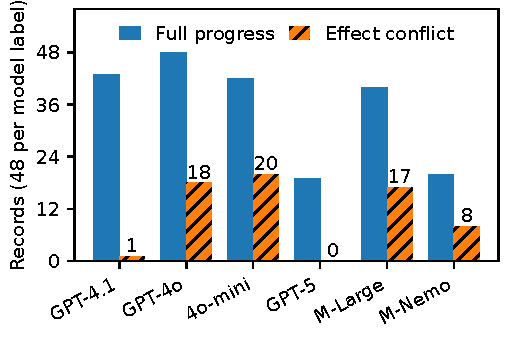
\includegraphics[width=\columnwidth]{figures/model_counts.pdf}
\caption{Reminder records by source model label: 48 per label across three templates. Right-hand bars count retained full-progress/effect conflicts, not an adjusted ranking. M-Large denotes \texttt{mistral\_large\_2411}; M-Nemo denotes \texttt{mistral\_nemo}.}
\label{fig:models}
\end{figure}

Conflicts occur under five model labels (Fig.~\ref{fig:models}). Of 144 reminder records per persona, expert users have 26 conflicts among 116 full-progress records; nonexpert users have 38 among 96. These are observational strata, not a causal comparison of user expertise. Four GPT-5-labelled candidates were legitimate rescheduling cases and were excluded; zero retained conflicts for that label is not a universal correctness claim.

\subsection{Concrete value and execution mismatches}
For the GPT-4o-labelled expert-user run in trial 2, the next-Friday task records a current epoch of 1758017684.319934 and a conversion receipt for Tuesday, September 16, 2025. The agent converts September 20 at 17:00 to 1758358800 and writes that value into the new reminder. September 20 is Saturday. The user does not reschedule, yet final source progress is one. Either candidate Friday interpretation rejects this stored date.

The same stratum contains a tomorrow task with current epoch 1758017671.957964 and created-reminder epoch 1697446800. The latter is in 2023, before the 2025 current clock. Thirty of the 62 calendar conflicts have reminder timestamps already in the past. No time-zone choice makes a past epoch tomorrow. The other conflicts include incorrect future dates or weekdays.

Two additional conflicts require different attribution. In one, an execution bridge forms a Python identifier beginning with a digit from a call ID and returns a syntax error before reminder creation. In the other, the assistant places an \texttt{add\_reminder}-like JSON object in ordinary text without a structured add call. Neither record contains the requested new reminder, but both have full source progress. We do not repair either trace or attribute the bridge error solely to model reasoning.

\subsection{Negative coverage and numerical verification}
The separate 960-record setting/contact coverage has 945 decidable local effects: 880 true and 65 false. All 802 decidable records with full source progress satisfy the checked effect. Thus we do not report a full-progress conflict in this coverage. One observed location-service reversal follows explicit permission to restore low-battery mode and has source progress 0.75; it is not counted as an unambiguous unauthorized full-score failure.

A separate implementation re-extracts clocks, conversion receipts, and final reminder tables from the original JSON rather than calling the primary predicates or reconstruction functions. It reproduces the 64 retained numerical/non-creation checks. The conservative weekday test also retains all 62 calendar conflicts. This checks numerical consistency, not independent agreement about user meaning. Original scores and raw records are preserved, and the public-data analysis does not replay the original serving environment.

\section{Native Temporal Controls}
\label{sec:controls}
To distinguish effect validity from historical achievement, we execute 45 scripted trajectories on eight unchanged public ToolSandbox tasks at commit \texttt{c8571d7}. Settings, contact updates, and reminder modification are represented. In each task, achieving the requested state and subsequently reversing it can still receive original similarity one, while the terminal effect is false. Normal completion, recovery after a non-mutating error, and repair after reversal remain positive controls. These eight counterexamples establish reachability in the evaluator, not a natural-agent incidence rate.

A further five traces use the public instruction to change initial friends to enemies and subsequently back to friends (Table~\ref{tab:scope}). Requiring both historical relationship targets at the final snapshot would reject the correct trace. Checking only the final friend state would accept inaction because that state was already true initially. Stage-scoped checks preserve the required first change and the authorized second change. The original evaluator accepts the correct revision but also accepts reversing the latest effect afterwards.

\begin{table}[t]
\centering
\caption{One public two-stage task: change initial friends to enemies, then back to friends. Scripted controls, not model samples. End checks only the latest friend state; scoped checks both required stages.}
\label{tab:scope}
{\fontsize{9}{10.8}\selectfont
\setlength{\tabcolsep}{3.5pt}
\begin{tabular}{@{}lccc@{}}
\toprule
Trajectory & Source & End & Scoped\\
\midrule
Both stages completed &1.0&Yes&Yes\\
Second update omitted &0.8&No&No\\
Latest effect reversed &1.0&No&No\\
No write; completion claims &0.6&Yes&No\\
No-op error, then both stages &1.0&Yes&Yes\\
\bottomrule
\end{tabular}}
\end{table}


These controls isolate a temporal measurement boundary. They do not explain the calendar conflicts: the latter generally never achieve the requested effect. The unchanged original ToolSandbox similarity and the public TED progress scores are never combined into one success metric. Code coverage over scripted counterexamples also does not demonstrate an improved autonomous agent or a general-purpose semantic verifier.

\section{Discussion and Limitations}
\label{sec:limits}
A stored object can exist with a wrong value; a plausible proposal can fail before execution; and a historical effect can legitimately expire or illegitimately be reversed. These require different evidence. Deterministic checks are appropriate for supported numeric relations, but cannot replace interpretation of a revised request or qualitative requirements.

The retained conflicts concern three reminder templates in one adaptation, using simulated users and source-reported models. Limited predicates do not certify all effects, and author review is not independent multi-rater annotation. Missing state, unresolved clock context, and ambiguous content remain unknown. We do not establish the cause of source judgments, quantify whole-dataset misalignment, or recompute TED's best-of-trial aggregates. In particular, the findings do not demonstrate a change in published model rankings or that cumulative progress caused the observed calendar errors.

\section{Conclusion}
ReCheck identifies 64 full-progress/effect conflicts in public saved agent records while retaining negative coverage and authorized-revision controls. The evidence supports a precise recommendation: audit completion claims against the active request, linked execution receipts, and actual effect values at the appropriate temporal boundary. This complements, rather than replaces, subgoal progress and path-flexible evaluation. The evidence is retrospective or explicitly scripted; it does not establish a model-performance gain.

\begin{thebibliography}{7}
\bibitem{toolsandbox}
J. Lu, T. Holleis, Y. Zhang, B. Aumayer, F. Nan, H. Bai, S. Ma, S. Ma, M. Li, G. Yin, Z. Wang, and R. Pang,
``ToolSandbox: A stateful, conversational, interactive evaluation benchmark for LLM tool use capabilities,''
in \emph{Findings of NAACL}, 2025, pp. 1160--1183, doi: 10.18653/v1/2025.findings-naacl.65.
\bibitem{ted}
P. Chong, H. Abichandani, J. Shen, A. Ghosh, M. P. Moe, Y. Mai, and D. Dahlmeier,
``Talk, Evaluate, Diagnose: User-aware agent evaluation with automated error analysis,''
in \emph{ICLR}, 2026. Also arXiv:2603.15483v1.
\bibitem{judge}
L. Zheng et al., ``Judging LLM-as-a-Judge with MT-Bench and Chatbot Arena,''
in \emph{Advances in Neural Information Processing Systems}, vol. 36, 2023. Also arXiv:2306.05685.
\bibitem{validity}
J. Vaghasiya, V. Bhat, M. A. Mohsin, and A. Aali,
``Benchmarking the benchmarks: A validity audit of tool-calling evaluation,''
\emph{arXiv preprint arXiv:2607.02577v1}, 2026.
\bibitem{aba}
J. Wang, F. Bianchi, S. Zhu, F. Nie, Y. Kwon, B. Dhingra, and J. Zou,
``Automated benchmark auditing for AI agents and large language models,''
\emph{arXiv preprint arXiv:2605.26079v2}, 2026.
\bibitem{timebench}
Z. Chu, J. Chen, Q. Chen, W. Yu, H. Wang, M. Liu, and B. Qin,
``TimeBench: A comprehensive evaluation of temporal reasoning abilities in large language models,''
in \emph{Proc. ACL}, 2024, pp. 1204--1228, doi: 10.18653/v1/2024.acl-long.66.
\bibitem{sapdata}
SAP, ``Agent Quality Inspect: Public experiment records,'' Hugging Face dataset, 2026,
revision \texttt{593e686} (full commit in the artifact manifest).
\url{https://huggingface.co/datasets/SAP/agent-quality-inspect}.
\end{thebibliography}

\end{document}
